\documentclass[article]{elsarticle}

\usepackage{lineno,hyperref}
\modulolinenumbers[5]

%% Nomenclature divided into different sections
\usepackage{framed}
\usepackage{mdframed}
\mdfdefinestyle{mdfexample1}{innerleftmargin=1cm,innerrightmargin=1cm,roundcorner=10pt,innertopmargin = 5pt, innerbottommargin = 5pt}

\usepackage{multicol} 
\usepackage[nonumberlist,nopostdot,nomain,automake]{glossaries}
\newglossary{v}{vas}{vao}{Variables}
\newglossary{s}{ses}{seo}{Sets}
\newglossary{p}{pas}{pao}{Parameters}
\newglossary{a}{aas}{aao}{Abbreviations}
\makeglossaries

%% Variables
\newglossaryentry{v1}{name =\ensuremath{CF_{t,s}}, description = {Fuel costs in year $t$ by ship $s$},type= v}
\newglossaryentry{v2}{name =\ensuremath{CI_{t,s}}, description = {Infrastructure costs in year $t$ by ship $s$},type= v}
\newglossaryentry{v3}{name =\ensuremath{CS_{t,s}}, description = {Ship costs in year $t$ by ship $s$},type= v}
\newglossaryentry{v4}{name =\ensuremath{fa_{t,s}}, description = {Fuel amount in year $t$ by ship $s$},type= v}
\newglossaryentry{v5}{name =\ensuremath{EC_{t,s}}, description = {CO$_2$ emissions in year $t$ by ship $s$},type= v}
\newglossaryentry{v6}{name =\ensuremath{EM_{t,s}}, description = {CH$_4$ emissions in year $t$ by ship $s$},type= v}
\newglossaryentry{v7}{name =\ensuremath{fainit_{t,s}}, description = {Initial fuel amount in year $t$ by ship $s$},type= v}
\newglossaryentry{v8}{name =\ensuremath{faicap_{t,s}}, description = {Infrastructure capacity in year $t$ by ship $s$},type= v}
\newglossaryentry{v9}{name =\ensuremath{fascap_{t,s}}, description = {Ship capacity in year $t$ by ship $s$},type= v}
\newglossaryentry{v10}{name =\ensuremath{faiup_{t,s}}, description = {Additional infrastructure capacity in year $t$ by ship $s$},type= v}
\newglossaryentry{v11}{name =\ensuremath{fasup_{t,s}}, description = {Additional ship capacity in year $t$ by ship $s$},type= v}

%% Sets
\newglossaryentry{s1}{name =\ensuremath{\mathcal{T}},description = {All time steps (years)},  type = s}
\newglossaryentry{s2}{name =\ensuremath{\mathcal{S}},description = {All ships},  type = s}
\newglossaryentry{s3}{name =\ensuremath{\mathcal{RO}(s)},description = {Refit option per ship type s},  type = s}
\newglossaryentry{s4}{name =\ensuremath{\mathcal{SNG}},description = {Ships not global-SECAs compliant},  type = s}
\newglossaryentry{s5}{name =\ensuremath{\mathcal{NT}},description = {Ships not NECAs compliant},  type = s}
\newglossaryentry{s6}{name =\ensuremath{\mathcal{SB}},description = {Ships burning bio-fuel},  type = s}
\newglossaryentry{s7}{name =\ensuremath{\mathcal{SR}},description = {Ships for short range},  type = s}
\newglossaryentry{s8}{name =\ensuremath{\mathcal{SNE}},description = {Ship not SECAs compliant},  type = s}


%% Parameters
\newglossaryentry{p1}{name =\ensuremath{cf_{t,s}},description={Fuel costs in year $t$ by ship $s$},type= p}
\newglossaryentry{p2}{name =\ensuremath{li_{t,s}},description={Infrastructure lifetime in year $t$ by ship $s$},type= p}
\newglossaryentry{p3}{name =\ensuremath{ci_{t,s}},description={Infrastructure costs in year $t$ by ship $s$},type= p}
\newglossaryentry{p4}{name =\ensuremath{ls_{t,s}},description={Ship lifetime in year $t$ by ship $s$},type= p}
\newglossaryentry{p5}{name =\ensuremath{cs_{t,s}},description={Ship costs in year $t$ by ship $s$},type= p}
\newglossaryentry{p6}{name =\ensuremath{ba_{t}},description={Bio-fuel availability in year $t$},type= p}
\newglossaryentry{p7}{name =\ensuremath{tdtotal_{t}},description={Total transport demand in year $t$},type= p}
\newglossaryentry{p8}{name =\ensuremath{tdshort_{t}},description={Transport demand on short range in year $t$},type= p}
\newglossaryentry{p9}{name =\ensuremath{tdnoneca_{t}},description={Transport demand outside ECAs in year $t$},type= p}
\newglossaryentry{p10}{name =\ensuremath{ts_{t,s}},description={Transport supply in year $t$ by ship $s$},type= p}
\newglossaryentry{p11}{name =\ensuremath{eb},description={Emission budget},type= p}
\newglossaryentry{p12}{name =\ensuremath{et},description={Emission target},type= p}
\newglossaryentry{p13}{name =\ensuremath{ec_{t,s}},description={CO$_2$ emissions in year $t$ by ship $s$},type= p}
\newglossaryentry{p14}{name =\ensuremath{em_{t,s}},description={CH$_4$ emissions in year $t$ by ship $s$},type= p}
\newglossaryentry{p15}{name =\ensuremath{slnonecayr},description={Inception year of global ECA},type= p}
\newglossaryentry{p16}{name =\ensuremath{tlecayr},description={Inception year of NECAs},type= p}

%% Abbreviations for math
\newglossaryentry{a1}{name = {ECA}, description={Emission control area},type= a}
\newglossaryentry{a2}{name = {SECA}, description={Sulphur emission control area},type= a}
\newglossaryentry{a3}{name = {NECA}, description={Nitrogen emission control area},type= a}

\usepackage{hyperref}
\makeatletter
\providecommand{\doi}[1]{%
  \begingroup
    \let\bibinfo\@secondoftwo
    \urlstyle{rm}%
    \href{http://dx.doi.org/#1}{%
      doi:\discretionary{}{}{}%
      \nolinkurl{#1}%
    }%
  \endgroup
}
\makeatother


\journal{Journal of \LaTeX\ Templates}

%% Additional packages
\usepackage{amsmath}
\usepackage{cleveref}
\usepackage{eurosym}
\usepackage{gensymb}
\usepackage{booktabs}
\usepackage{caption}

%%%%%%%%%%%%%%%%%%%%%%%
%% Elsevier bibliography styles
%%%%%%%%%%%%%%%%%%%%%%%
%% To change the style, put a % in front of the second line of the current style and
%% remove the % from the second line of the style you would like to use.
%%%%%%%%%%%%%%%%%%%%%%%

%% Numbered
%\bibliographystyle{model1-num-names}

%% Numbered without titles
%\bibliographystyle{model1a-num-names}

%% Harvard
%\bibliographystyle{model2-names.bst}\biboptions{authoryear}

%% Vancouver numbered
%\usepackage{numcompress}\bibliographystyle{model3-num-names}

%% Vancouver name/year
%\usepackage{numcompress}\bibliographystyle{model4-names}\biboptions{authoryear}

%% APA style
%\bibliographystyle{model5-names}\biboptions{authoryear}

%% AMA style
%\usepackage{numcompress}\bibliographystyle{model6-num-names}

%% `Elsevier LaTeX' style
\bibliographystyle{elsarticle-num}
%%%%%%%%%%%%%%%%%%%%%%%

\begin{document}

\begin{frontmatter}

\title{Future Marine Fuels - A Danish Case Study on Climate Compatible Energy Pathways}
%\tnotetext[mytitlenote]{Fully documented templates are available in the elsarticle package on %\href{http://www.ctan.org/tex-archive/macros/latex/contrib/elsarticle}{CTAN}.}

%% Group authors per affiliation:
\author[label1]{Till ben Brahim\corref{cor1}}
\address[label1]{Technical University of Denmark, Produktionstorvet, Bygning 426, 2800 Kongens Lyngby, Denmark}
\ead{tilseb@dtu.dk}

\cortext[cor1]{Corresponding author}

\author[label1]{Frauke Wiese}
\ead{frwi@dtu.dk}

\begin{abstract}
This template helps you to create a properly formatted \LaTeX\ manuscript.
\\
This research did not receive any specific grant from funding agencies in the public, commercial, or
not-for-profit sectors.
\end{abstract}

\begin{keyword}
% \texttt{elsarticle.cls}\sep \LaTeX\sep Elsevier \sep template
% \MSC[2010] 00-01\sep  99-00
Maritime transport\sep Marine fuels\sep Energy modelling\sep Emission reduction\sep Danish case-study 
\end{keyword}

\end{frontmatter}

\linenumbers

\section{Introduction}
% 1000
% The journal covers research in mechanical engineering and thermal sciences, with a strong focus on energy analysis, energy modelling and prediction, integrated energy systems, energy planning and energy management.

% What is required from the climate side and what does the IMO suggest so far
The ambition to reach climate pathways with limited overshoot of 1.5~\degree C requires global net zero CO$_2$ emissions by 2050 \cite{IPCC2018}. This implies a massive reduction of fossil fuels in the energy system. Several studies based on energy system models have shown possible pathways to net zero emissions for the electricity supply from country to continents and the whole world (TODO:references) and also for the heat sector. Although transport is more challenging (TODO:cite), in recent years an increasing amount of studies also includes pathways for this sector to net zero emissions in 2050 (TODO:cite). Though, the majority of scenarios leaves out a significant part of the transport emissions, namely international shipping (TODO:CITE?). Due to its international nature, appropriate governance is challenging \cite{GRITSENKO2017}. So far, countries leave out international shipping in their energy and climate plans, leaving the responsibility to the International Maritime Organisation (IMO). While -- to some extent -- progress has been made regarding sulphur emission reduction, their goal of at least 50\% reduction until 2050 of worldwide shipping \cite{IMO2018} is neither ambitious enough to reach the goals of the Paris Agreement, nor underpinned with measures and possible pathway descriptions \cite{Wan2018}.

% Concentration on sulphur etc. does not lead further, just concentrating on LNG is too shortsighted
While liquefied Natural Gas (LNG) has mainly been in the focus as an alternative marine fuel \cite{IMO2016a,DNVGL2015} due to its advantage regarding sulphur, NO$_x$ and particle emissions, its possibility to also reduce climate impact of shipping has increasingly be questioned \cite{BRYNOLF2014b}. This is on the one hand due to its limited CO$_2$ emission benefit compared to oil \cite{DNVGL2014}. On the other hand, the implications for greenhouse gases depend on how the natural gas is extracted, processed, distributed, and used \cite{THOMSON2015}. According to IEA \cite{IEA2017}, average global gas methane leakage rate is almost 2~\% for natural gas. Looking at a global warming potential over a 20-year time frame, a leakage rate of 3-4~\% would already use up the climate benefit of natural gas compared to coal, over a 100-year time frame 6-7~\%. \citep{Hagos2018} states that a 1~\% methane slip from a dedicated LNG passenger vessel results, on average, in 8.5~\% increase in net GHG emissions. According to measurements and calculations based on \cite{Corbett2015,Stenersen2017}, methane slip of dual-fuel engines amounted to roughly 4~\% and of dedicated gas engines to 2.3~\% in 2016. Although LNG-specialised engines with high pressure direct injection could could lower leakage rates even further, ship owners today prefer dual-fuel engines as they judge flexibility and the resale value of the ship more important than efficiency gains because climate impact is not reflected in any economic value for shipping. 
In summary, the climate impact of both, LNG and methanol produced from natural gas is on the same order of magnitude as with use of heavy fuel oil \cite{BRYNOLF2014,DNVGL2018}. 
Independent of the role of LNG, one can generally conclude, that the current concentration on reduction of sulphur, NO$_x$ and particle emissions in shipping is too short-sighted \cite{Gilbert2014}, since climate emissions from shipping are the bigger challenge \cite{FRIDELL2019}. More radical changes avoiding infrastructure lock-ins and exploring co-benefits of sulphur and carbon reduction are advisable.

% So, what else than LNG could one do? - Some studies with different fuels in the focus
In line with that, the discussion about climate and other emission compatible future marine fuels has gained momentum in recent years. Indirect electrification via hydrogen or other synthetic fuels could be a promising option \cite{HORVATH2018} if relying on decarbonised inputs as well as bio-derived fuels under circumstances related to its scarcity \cite{Gilbert2014}. Also wind-energy in form of soft-sails, fixed-sails, Flettner Rotors or kite sails are options tested \cite{IRENA2015}.
% Specifically on hydrogen \cite{Raucci2017}. And methanol \cite{IMO2016b} with one big ferry already driving on it.

% and studies with other measures to reduce emissions
Another important aspect of reducing emissions additionally to fuel switch is energy efficiency measures, which are not completely exploited yet \cite{JAFARZADEH2014,CHI2018} and could be further improved applying e.g. waste heat recovery \cite{Baldi2015}. Furthermore, operational measures like slow steaming \cite{ARMSTRONG2013}, hull design and larger vessels \cite{LINDSTAD2015} can provide significant contributions to lowering emissions in shipping. However, as \cite{Olmer2017} show, shipping will need to move beyond energy efficiency interventions alone to achieve absolute emission reductions.

% But operational measures are not enough, we need a mixture.
Calculating different pathways until 2050, \cite{LloydsRegister2016} come to the conclusion, that different options are possible, mostly depending on the availability of biomass, the development of transport demand and technology learning, but in dependant of the pathway, all require a substitute for fossil fuel, operational measures are not sufficient. A meta-study looking at measures and fuels of various studies \cite{Bouman2017}, comes to the conclusion that a  75\% emission reduction is possible until 2050, but only with combination of measures. Looking at possible reduction targets, \cite{Smith2016} describe the pathway to zero emissions in 2035 in their most ambitious scenario. There is also an initiative from the shipping industry itself, striving for zero emission vessels \cite{SSI2018}, also worked on by Lloyd Register \cite{LloydsRegister2017}. 

% some studies rather for specific technologies, or on local level
Additionally to studies taking the meta-perspective, there is ongoing research about specific applications, like e.g. batteries in offshore support vessels \cite{Lindstad2017}, specific fuel options, like e.g. slow steaming and wind propulsion \cite{MANDER2017} or specific areas like emission reduction in port \cite{WINNES2015}.
% maybe add or for e.g. electric ferries in Denmark (TODO:cite)

% Regulation
Looking at the regulative side, \cite{SHI2016} suggests a scheme of market-based measures that can be adopted by means of an international convention under the auspices of the IMO and the UNFCCC. This could be a global emission trading scheme including shipping and aviation \cite{Dessens2014}, while \cite{GRITSENKO2017} suggests polycentric governance \cite{},

% Why it is so bad that shipping is underrepresented in the current discussion
Although at least in the scientific discussion, the technical, economical and regulative options for shipping to take its share in the climate responsibility has risen, it is still under-represented in current discussions and studies assessing energy transformation, regarding its importance and urgency. Its importance is due to (1) the general efficiency of shipping compared to other means of transport (TODO:citeAndNumber), (2) large share in worldwide transported goods (TODO:number and cite) and (3) wide range of transport demand predictions. According to the upper bound of predictions future cargo transport demand would increase by (TODO:citeAndNumber), which would heavily increase emissions as well. However, other predictions even assume a decrease in transport demand due to less fossil fuel transported, as well as increased circular economy and effects from 3D-printing (TODO:cite).

The urgency is due to (1) very long investment cycles of ships. This leads to the situation that decisions about the fuels to reach net zero emissions in 2050 are just around the corner. (2) Infrastructure requirements being essential and (3) the increasing interdependence between fuels applied in shipping and our land-based energy systems (electricity, heat, fuels for transport). Developments in shipping fuels will affect decisions on energy infrastructure on land and vice versa. Examples are refineries providing fuels for shipping but also land-based heavy transport, producing excess heat during the fuel production. Thus, options have to be intensively looked at and also optimised in combination with the rest of the energy system. 
% Maybe add example biomass scarcity - where to use the scarce biomass best?

% Which gap does this paper close?
% closing gap between international and local studies
This paper contributes to fill the gap between studies on inland shipping  with a high level of detail but limited scope and international shipping in low resolution regarding technology- and fuels. Our modelling approach takes emissions from international shipping into account but can be applied for single or several countries. It could thus be integrated in national energy and climate modelling scopes. Although we exemplary model Danish shipping, the methodology could be applied to other countries as well.
% taking the different costs and emissions into account
Unlike most other studies, data and model not only include costs for fuels and technologies but also infrastructure costs. Emission-wise, the whole picture is covered by taking well-to-propeller climate emissions including methane leakage into account while complying with current and future sulphur, NO$_x$ and particle emission restrictions.
% Several scenarios and threshold analysis regarding technology, fuel and infrastructure costs
In this holistic approach, today's and possible alternative fuels and technologies are evaluated against each other by an optimisation model, minimising total system costs while reaching net zero emissions in 2050. Due to high uncertainty regarding cost development, we perform a threshold analysis providing an overview of fuels-technology combinations likely to play a role in the future.

% What the reader can expect
In \autoref{sec:Methods}, we describe the mathematical formulation (\autoref{subsec:Mat}), data sources and processing (\autoref{subsec:Dat})and give and explain our scenario approach (\autoref{subsec:Sce}. Subsequently, we present the scenario and threshold analysis results and discuss their relevance, also describing strengths and weaknesses of the model approach (\autoref{sec:Results} and finally conclude (\autoref{sec:Conclusion}).  

\section{Materials and Methods}
\label{sec:Methods}
% 1500-1750

\subsection{Model Scope}
The model consists of different scopes and dimensions which mutually influence their degrees of freedom. The temporal scope of the model ranges from the initial year 2016 to 2050 with annual resolution. In the spatial dimension annually aggregated sailing routes to and from Danish ports are considered. In order to allocate the responsibility for negative external effects that, as for now, inevitably accompany the international maritime shipping in a fair manner to both trading entities countries, cross-border connections account with have of their total estimated distances (see \cref{fig:model_boundary}). A further dimension taken into account is the system's economy in terms of expenditures into infrastructure, ships and fuels. The model identifies identifies depreciated system components and undertakes investment decisions accordingly. Fixed investments are either for the fuel infrastructure or new ships, while the annual fuel amounts to supply the full fleet are considered variable. The technical dimension is set by the considered ship types, which are solely distinguished by their power systems as a combination of main engine and fuel type. All other ship specific design characteristics like hull-shapes or operational patterns (e.g. sailing speeds) are neglected. The complete set of ships available to the model can be found in \cref{tab:ship_data}. The emission dimension is composed of global and regional legislation on the one and GHG effective emissions on the other hand. SOx and NOx emissions are legally restricted by the Marpol Annex VI regulations 13 and 14 on global and regional scale \cite{IMO2008a,IMO2008b}. As for GHG emissions, CO2 and CH4 are regarded and subject to different limitations, depending on the scenario. In general, CO2e emissions are constraint by an overall budget and 2050 target that are derived from the IPCC's RCP2.6 pathway aiming at a maximum surface temperature increase of 1.5 degrees Celsius compared to pre-industrial levels \cite[p.~27]{IPCC2013}.

\begin{figure}[htb]
    \centering
    \includegraphics[width=\textwidth]{figures/model_boundary_paper.pdf}
    \caption{Model boundary: The model considers the specifications inside the green box.}
    \label{fig:model_boundary}
\end{figure}

\subsection{Model Structure}
Technically, the model consists of two different components. Firstly, instances, secondly processes to manipulate instances. In the present case instances hold numerical and literal data in table format. Processes in turn are the formal operational instructions translated into a software language, here Python is used. The two components alternate throughout the model flow like a cascade. In the model box-flow in \cref{fig:model_boxflow} white boxes represent data instances, whereas the blue arrows represent processes. An entire model run for a selected scenario starts by loading the technology data, incorporating scenario specifications and creating the model input files. In the course of generating the model, these input files are translated into parameters and sets. The solver then calculates the model variables based on their degrees of freedom, which are determined by the the input data and the sense of the model objective. The results are stored again as data instances in the output directory. To allow for interpretations of the results, the post-processing provides edited graphical and tabular data.

\begin{figure}[tbh]
    \centering
    \includegraphics[width=\textwidth]{figures/model_boxflow_paper.pdf}
    \caption{Model boxflow: The core model consists of the components inside the green box.}
    \label{fig:model_boxflow}
\end{figure}

\subsection{Mathematical Formulation}
\label{subsec:Mat}
The problem is formulated in a linear, divisible manner, aiming to minimise the objective function. It is a stock model, initialised with data for the first time step and allows for investments in new technologies in the further course. Investment decisions are on the one hand forced and on the other limited by the model constraints that in general reflect legal frameworks and behaviour patterns of the investigated system. Since the objective's sense is the minimisation of the overall total system's costs \cref{eq:objective}, investments are interpreted as adverse, yet inevitable actions to cope with the constraint's demands, such as: Lowering CO$_2$e emissions to air, (over-)supplying the transport demand in each time step or scrapping ships. All model variable's domains are within non-negative real numbers, including zero $\left(R_{0}^{+}\right)$. The nomenclature used in the equations and table headers in the following sections is given in the nomenclature list.
\glsdisablehyper
\glsaddall
\begin{table*}[thb] 
\renewcommand\tablename{Nomenclature list}
\begin{mdframed}
\footnotesize{
%\begin{mdframed}[style=mdfexample1]
\begin{multicols}{2}
\printglossary[style=tree,type=a]
\vspace{-0.3cm}
\printglossary[style=tree,type=s]
\vspace{-0.3cm}
\printglossary[style=tree,type=v]
\vspace{-0.3cm}
\printglossary[style=tree,type=p]
\end{multicols}
}
\end{mdframed}
\caption{}
\end{table*}

\subsubsection{Objective function}
The model's objective is the minimisation of the total system costs over all time steps and ship types. It comprises accumulated annual costs for fuel, infrastructure and ships. Fixed cost components account only with the annual added amounts and are multiplied with their respective lifetimes, since they are given to the model as annuities. The stock of fixed assets present in 2016 ($fainit_{t,s}$ in $T_0$) is not cost-effective and therefore subtracted from $CI$ and $CS$.
\begin{subequations}
    \begin{align}
        min. &\sum_{\forall t \in T}\sum_{\forall s \in S}\left( CF_{t, s} + CI_{t, s} + CS_{t, s} \right)\label{eq:objective}\\
        \intertext{s.t.}
        CF_{t, s} &\geq fa_{t,s} \cdot cf_{t,s}\\
        CI_{t, s} &\geq \left( faiup_{t,s} - fainit_{t, s} \right) \cdot li_{s} \cdot ci_{t,s}, \forall t \in T_0\\
        CI_{t, s} &\geq faiup_{t,s} \cdot li_{s} \cdot ci_{t,s}, \forall t \in T_{>0}\\
        CS_{t, s} &\geq \left( fasup_{t,s} - fainit_{t, s} \right) \cdot ls_{s} \cdot cs_{t,s}, \forall t \in T_0\\
        CS_{t, s} &\geq fasup_{t,s} \cdot ls_{s} \cdot cs_{t,s}, \forall t \in T_{>0}
    \end{align}
\end{subequations}

\subsubsection{Fuel constraints}
The following fuel constraints refer to the amounts of fuel per ship type in each time step. Investments in infrastructure, new-build and refitted ships consider exclusively the sum of the additional capacities per ship or infrastructure over the respective lifetime. Ships and infrastructure are separated, due to different costs and lifetimes, even if they belong to the same technology.\\\par\noindent
\textit{Infrastructure capacity: }Sum of all added infrastructure capacity within the respective proceeded technical lifetime.
\begin{subequations}
    \begin{align}
        faicap_{t,s} &\leq \sum_{\textbf{x}}^{t-1} \left( faiup_{x,s} \right), \forall t \in T_{>0}, \forall s \in S\label{eq:faicap}\\
        \intertext{s.t.}
        x &= T_0, \forall t \leq \left(li_{s} + T_0 - 1\right)\\
        x &= t - li_{s} + 1, \forall t > \left(li_{s} + T_0 - 1\right)
    \end{align}
\end{subequations}\\
\textit{Additional infrastructure: }Annual additional infrastructure capacity needed to (over-)supply the fleet.
\begin{equation}
    faiup_{t,s} \geq fa_{t,s} - faicap_{t,s}, \forall t \in T_{>0}, \forall s \in S\label{eq:faiup}
\end{equation}\\
\textit{Ship capacity: }Sum of all added ships within the respective proceeded technical lifetime.
\begin{subequations}
    \begin{align}
        fascap_{t,s} &\leq \sum_{\textbf{x}}^{t-1} \left(fasup_{x,s} \right), \forall t \in T_{>0}, \forall s \in S\label{eq:fascap}\\
        \intertext{s.t.}
        x &= T_0, \forall t \leq \left(ls_{s} + T_0 - 1\right)\\
        x &= t - ls_{s} + 1, \forall t > \left(ls_{s} + T_0 - 1\right)
    \end{align}
\end{subequations}\\
\textit{Added ships: }Annual additional ship capacity needed to (over-)supply the transport demand.
\begin{equation}
    fasup_{t,s} \geq fa_{t,s} - fascap_{t,s}, \forall t \in T_{>0}, \forall s \in S\label{eq:fasup}
\end{equation}\\
\textit{Ship refit: }Defines for each time step the maximum fuel amount available for the refit of old ships.
\begin{subequations}\label{eq:refitships}
    \begin{align}
    fa_{t,s} + fa_{t,r} - fa_{T_0, s} &\leq 0, \forall t \in T_{<\left(T_0+ls_{s}\right)}, \forall s, r \in RO\\
    fa_{t,s} + fa_{t,r} & = 0, \forall t \in T_{\geq\left(T_0+ls_{s}\right)}, \forall s, r \in RO
    \end{align}
\end{subequations}\\
\textit{Bio-fuel availability: }Defines for each time step the maximum bio-fuel availability.
\begin{equation}
    \sum_{\forall s \in SB} \left(fa_{t,s} \right) - ba_{t} \leq 0, \forall t \in T\label{eq:biofuel}
\end{equation}

\subsubsection{Demand constraints}
The following demand constraints refer to the amounts of fuel per transport demand type. These types are either defined by the sailing distance (short or long) and location (ECAs or not).\\\par\noindent
\textit{Total transport demand: }The sum of all annual transport supply per ships must be greater or equal to the total transport demand in each time step.
\begin{equation}
    tdtotal_t \leq \sum_{\forall s \in S} \left( fa_{t,s} \cdot ts_{t,s}\right), \forall t \in T \label{eq:td_total}
\end{equation}
\textit{Short transport demand: }The amount of fuel available for short range shipping is limited by the transport demand of that range.
\begin{equation}
    tdshort_t \geq \sum_{\forall s \in SR} \left( fa_{t,s} \cdot ts_{t,s}\right), \forall t \in T \label{eq:td_short}
\end{equation}
\textit{Non-SECAs transport demand: }Defines the maximum amount of fuel available for shipping not in compliance with sulphur regulations, which comprises all transport demand outside of the SECAs.
\begin{equation}
    tdnoneca_t \geq \sum_{\forall s \in SNE} \left( fa_{t,s} \cdot ts_{t,s}\right), \forall t \in T \label{eq:td_noneca}
\end{equation}

\subsubsection{Emission constraints}
The set of emission constraints imposes limitations to the extend of which certain fuel types are being deployed by the model, based on the CO2e budget and target as well as the legal restrictions defined by the IMO.
\\\par\noindent
\textit{Emission budget: }The emission budget must be greater or equal to the total systems well-to-propeller CO2e emissions.
\begin{subequations}
    \begin{align}
    eb &\geq \sum_{\forall t \in T}\sum_{\forall s \in S}\left(EC_{t,s} + EM_{t,s} \right) \label{eq:co2ebudget}\\
    \intertext{s.t.}
    EC_{t,s} &= fa_{t,s} \cdot ec_{t,s}, \forall t \in T, \forall s \in S\\
    EM_{t,s} &= fa_{t,s} \cdot em_{t,s}, \forall t \in T, \forall s \in S
    \end{align}
\end{subequations}\\
\textit{Emission target: }Limits the CO2e emissions from the selected year (2050) on-wards.
\begin{equation}
    \frac{\sum_{\forall s \in S} \left(EC_{T_0,s}+EM_{T_0,s}\right)}{\sum_{\forall s \in S} \left(EC_{t,s}+EM_{t,s}\right)} \cdot et \geq 1, \forall t \in T_{\geq \left(etyr-T_0\right)}
\end{equation}\\
\textit{Global SOx regulations: }From the year 2020 on-wards the fuel amount of those ship types is set to zero, whose sulphur content exceeds the global sulphur limit and have no scrubber installed.
\begin{equation}
    fa_{t,s} = 0, \forall t \in T_{\geq slnonecayr-T_0}, \forall s \in SNG \label{eq:sox_global}
\end{equation}\\
\textit{NECAs regulations: }Sets the fuel amount to zero for ships not in compliance with the NOx regulations inside the EU-NECAs from 2021 on-ward.
\begin{equation}
   fa_{t,s} = 0, \forall t \in T_{\geq tlecayr-T_0},\forall s \in NT \label{eq:tier}
\end{equation}


\subsection{Data}
\label{subsec:Dat}
The fuel and ship data tables contain both, information about the status-quo of the Danish maritime industry and future investment options for alternative means of shipping. For fuel data the unique identifier is the fuel type, for ship data it is ship type. Ship types can use the same fuel type, but then use a different engine type (IC, FC, EM).

\subsubsection{Fuel data}
The set of fuel technology parameters ranges from fuel and infrastructure costs, over well-to-tank CO2e emission operation factors and sulphur contents to the fuel infrastructure's technical lifetimes (\cref{tab:fuel_data}). Regarding fuel costs, it is assumed that the bunker index prices of the currently available fuels (HFO, MDO, BDO) comprise all upstream cost components from well-to-tank. Thus, the fixed costs of the supply chain are incorporated (e.g. sufficient supply infrastructure). In contrast, new fuel technology costs are divided into fixed and variable components, since sufficient supply infrastructure has not been installed. When upgrading facilities are required, they are assumed to be placed directly at the port, so that additional fuel transport infrastructure is eluded. Further, upon consultation with Danish transmission grid operator EnergiNet, the gas transmission grid is assumed to cope with any conceivable additional demand for natural or upgraded bio-gas transport.
\begin{table}[htb]
    \centering
    \resizebox{\textwidth}{!}{
    \begin{tabular}{lrrrrrrr}
        \toprule
        Fuel type & cf & ci & ec(w2t) & em(w2t) & sulphur content & li & References \\
        & $\left[\frac{EUR_{2016}}{GJ_{fuel}}\right]$ & $\left[\frac{EUR_{2016}}{GJ_{fuel}}\right]$ & $\left[\frac{g_{co2}}{MJ_{fuel}}\right]$ & $\left[\frac{g_{ch4}}{MJ_{fuel}}\right]$ & $\left[\%_{mass}\right]$ & $\left[a\right]$ & \\
        \midrule
        HFO   & \multicolumn{2}{c}{6.547} & 8.148      & 0.090            & 2.9525   & 40   & \cite{BIX2018,Gilbert2018,Bengtsson2012,BRYNOLF2014}    \\
        MDO   & \multicolumn{2}{c}{12.775} & 7.728     & 0.090            & 0.7500   & 40   & \cite{BIX2018,Gilbert2018,Bengtsson2012,Andersson2015}    \\
        BDO   & \multicolumn{2}{c}{24.240} & 0         & 0.030            & 0.1498   & 40   & \cite{SSI2018,Bengtsson2012}    \\
        LNG   & 4.888    & 0.139    & 6.600            & 0.033            & 0.0500   & 36   & \cite{EnerginNet2018,Gilbert2018,BRYNOLF2014,Andersson2015}    \\
        LBG   & 27.847   & 1.599    & 0                & 0.130            & 0.0750   & 25   & \cite{Brynolf2018,Bengtsson2012}    \\
        H2    & 20.885   & 1.199    & 0                & 0                & 0        & 25   & \cite{Brynolf2018}    \\
        CH3OH & 29.240   & 1.679    & 0                & 0.042            & 0.0912   & 25   & \cite{Brynolf2018,BRYNOLF2014}    \\
        NH3   & 26.803   & 1.802    & 0                & 0                & 0        & 20   & \cite{Morgan2017}    \\
        ELEC  & 13.889   & 2.929    & 0                & 0                & 0        & 20   & \cite{Vree2008}    \\
        \bottomrule
    \end{tabular}}
    \caption[Fuel type data]{Fuel type data for each parameter.}
    \label{tab:fuel_data}
\end{table}

\subsubsection{Ship data}
Compared to the fuel's category set, the ship's set is more divers. This is because of technical information needed to distinguish the different ship types and applying relevant regulative and technical constraints. The fuel specific parameters range from transport supply, over investment costs to the tank-to-propeller CO2e emission operation factors. Further, initial fuel amounts per ship type are provided (see \cref{tab:ship_data}). Transport demand in the first year is equal to the sum-product of fuel amount and ship specific transport supply, whilst future fuel amounts are calculated by the model. Technical categories complement the parameter set. Firstly, the sailing range classification, which is unlimited for all but full electric ships. It is followed by the ship's technical lifetime. For old ships, the average remaining lifetime is 11 years. as the average age of the current fleet is 14 years, when considering the three main Danish cargo ship types bulker, containers and tankers listed in \cite[Tab.~2.2, p.~27]{UNCTAD2017} and combined with their market shares based on own assumptions with regard to cargo types. Information about refit possibility, Tier rating and scrubber installation complete the set.


Refits are build upon existing ships. Ship with internal combustion engines that run on HFO can be refitted with scrubber. When operating with a scrubber SOx emissions are reduced. However, the downside is a loss in transport supply capability, since the scrubber impairs the ship's energy efficiency. Refitting old ships with an internal combustion engine towards the use of BDO has no associated major investment costs. Note, that the refit measures have no effect on the ships lifetime. The model simply transfers the residual lifetime of the old ship to the one refitted. Consequently, the technical lifetime provided for refitted ships in \cref{tab:ship_data} is just the maximum value. Based on the IMO's NOx regulations, Tier levels are decisive for ship operations in the NECAs. All new-build ships have the Tier 3 rating as they are being constructed later than 2016. In contrary, old ships have no or a Tier rating of 1, as the average construction year was in 2002. Here, no rating is selected. Hence, old ships will either be scrapped after 2021 or need a refit to gain a higher rating.
\begin{table}[htb]
    \centering
    \resizebox{\textwidth}{!}{
    \begin{tabular}{llrrrrrrrrrrr}
        \toprule
                       Ship-type & Range & ls & fa$_{2016}$ & ts & cs & ec(t2p) & em(t2p) & Refit & Refit opt. & Tier & Scrubber & References \\
                       &       & $\left[a\right]$ & $\left[PJ_{fuel}\right]$ & $\left[\frac{Ttkm}{GJ_{fuel}}\right]$ & $\left[\frac{EUR_{2016}}{GJ_{fuel}}\right]$ & $\left[\frac{g_{CO2}}{MJ_{fuel}}\right]$ & $\left[\frac{g_{CH4}}{MJ_{fuel}}\right]$ & & & & & \\
        \midrule
        IC HFO (old)   & long  & 11     & 9.93   & 9.69        & 8.72     & 76.06            & 0.00045          & yes   & IC HFO (refit) & 0           & no     & \cite{UNCTAD2017,Eurostat2018,Wisdom2017,Kristensen2012,Rex2017} \\
        IC MDO (old)   & long  & 11     & 5.99   & 9.40        & 8.45     & 74.36            & 0.00045          & yes   & IC BDO (refit) & 0           & yes    & \cite{UNCTAD2017,Eurostat2018,Wisdom2017,Kristensen2012,Rex2017} \\
        IC HFO         & long  & 25     & 0      & 9.40        & 8.45     & 75.90            & 0.00045          & no    &                & 3           & yes    & \cite{UNCTAD2017,Kristensen2012,Rex2017} \\
        IC MDO         & long  & 25     & 0      & 9.40        & 8.45     & 74.32            & 0.00045          & no    &                & 3           & yes    & \cite{UNCTAD2017,Kristensen2012,Rex2017} \\
        IC HFO (refit) & long  & 11     & 0      & 9.40        & 0.02     & 75.90            & 0.00045          & no    &                & 3           & yes    & \cite{UNCTAD2017,McGill2013} \\
        IC BDO (refit) & long  & 11     & 0      & 9.40        & 0        & 0                & 0.00045          & no    &                & 3           & yes    & \cite{UNCTAD2017,Wisdom2017} \\
        IC BDO         & long  & 25     & 0      & 9.40        & 8.45     & 0                & 0.00045          & no    &                & 3           & yes    & \cite{UNCTAD2017,Bengtsson2012} \\
        IC LNG         & long  & 25     & 0      & 10.13       & 96.98    & 54.36            & 0.71000          & no    &                & 3           & no     & \cite{UNCTAD2017,Kristensen2012,Rex2017} \\
        IC LBG         & long  & 25     & 0      & 10.13       & 96.98    & 0                & 0.79000          & no    &                & 3           & no     & \cite{UNCTAD2017,Bengtsson2012} \\
        IC H2          & long  & 25     & 0      & 10.13       & 109.29   & 0                & 0                & no    &                & 3           & no     & \cite{UNCTAD2017,ElGohary2013} \\
        IC CH3OH       & long  & 25     & 0      & 10.13       & 109.29   & 0                & 0.79000          & no    &                & 3           & no     & \cite{UNCTAD2017,Andersson2015,BRYNOLF2014} \\
        IC NH3         & long  & 25     & 0      & 10.13       & 109.29   & 0                & 0                & no    &                & 3           & no     & \cite{UNCTAD2017} \\
        FC LNG         & long  & 25     & 0      & 22.47       & 134.80   & 54.36            & 0.22763          & no    &                & 3           & no     & \cite{UNCTAD2017,VanBiert2016} \\
        FC LBG         & long  & 25     & 0      & 22.47       & 134.80   & 0                & 0.22763          & no    &                & 3           & no     & \cite{UNCTAD2017,VanBiert2016} \\
        FC H2          & long  & 25     & 0      & 22.47       & 134.80   & 0                & 0                & no    &                & 3           & no     & \cite{UNCTAD2017,USDE2015} \\
        FC CH3OH       & long  & 25     & 0      & 22.47       & 134.80   & 0                & 0.22763          & no    &                & 3           & no     & \cite{UNCTAD2017,VanBiert2016} \\
        FC NH3         & long  & 25     & 0      & 22.47       & 134.80   & 0                & 0                & no    &                & 3           & no     & \cite{UNCTAD2017} \\
        EM ELEC        & short & 30     & 0      & 11.86       & 1,047.05 & 0                & 0                & no    &                & 3           & no     & \cite{DNVGL2015} \\
        WIND ELEC      & long  & 30     & 0      & 35.58       & 2,094.11 & 0                & 0                & no    &                & 3           & no     &  \\  
    \bottomrule
    \end{tabular}}
    \caption[Ship type data]{Ship type data for each specific parameter.}
    \label{tab:ship_data}
\end{table}

\subsubsection{Emission budget}
The CO2e emission budget sets a limit to the total allowed GHG emissions to air over the full temporal model scope. The Danish budget is derived from a global emission budget estimate by the IPCC \cite[Tab.~SPM.3, RCP2.6]{IPCC2013} and the global maritime budget share, provided by the ICCT \cite{Olmer2017}.

Comparison of global maritime CO2e emissions in 2012 with the Danish emissions in 2016 and its application to the global maritime budget leads to the Danish GHG budget. The absolute level of Danish cargo shipping emissions of 1.2 Mt CO2e in 2016 is derived from the fuel specific emission operation factors, multiplied by total fuel consumed in that year. Comparing maritime emissions from 2012 and 2016 can be considered a conservative estimation, as global maritime trade volume has increased over this period \cite[Tab.~1.3,~p.~5]{UNCTAD2017}. Thus, the Danish budget would be lower by the same proportion. Keeping this emission level constant would deplete the budgets within the next 15 years and is more ambitious than just a linear decrease of emissions from 2016 to 2050.
\begin{table}[htb]
    \centering
    \begin{tabular}{llrr}
        \toprule
         & Unit & CO2e emissions & References \\
         \midrule
         Global budget & $\left[Gt\right]$ & 510 & \cite{IPCC2013} \\
         Global maritime budget share & $\left[\%\right]$ & 3 & \cite{Olmer2017} \\
         Global maritime budget & $\left[GT\right]$ & 15.3 &\\[1.5ex]
         Global maritime emissions in 2012 & $\left[Mt\right]$ & 961 & \cite{Smith2014} \\
         Danish maritime emissions in 2016 & $\left[Mt\right]$ & 1.2 & \cite{Kristensen2012,Eurostat2018,Wisdom2017} \\
         Danish maritime emission share & $\left[\%\right]$ & 0.125 &\\[1.5ex]
         Danish budget & $\left[Mt\right]$ & \textbf{19.12} & \\
         \bottomrule
    \end{tabular}
    \caption[Danish CO2e emission budget]{Derivation of CO2e emission budget from global to Danish level.}
    \label{tab:dk_em_budget}
\end{table}


\subsection{Scenarios}
\label{subsec:Sce}


\subsubsection{Scenario data}
The scenario data set consists of fuel rates, ship rates and regulative limits. Assuming that model parameters are not necessarily constant over all time steps some parameters are subject to variation. The variations are given as the total percentage change between 2016 and 2050. This difference is translated into a constant annual changing rate. Therefore, the change is not linear but exponential. With this, time dependent parameters are created. The reference scenario provides the baseline rates and limits. When a different scenario is calculated, the final value in 2050 of a selected parameter can be alternated by any percentage. Though, the minimum threshold is -100 \%, that would correspond to a reduction towards zero costs or no limitations.

\begin{table}[htb]
    \centering
    \resizebox{\textwidth}{!}{%
    \begin{tabular}{lrcr}
        \toprule
        Modified Parameters & Change to 2050 & Affected Technologies & References \\
        \midrule
        ic  & -20   & LNG,LBG,H2,CH3OH,NH3,ELEC         & \cite[fig.~6,~p.~13]{Brynolf2018}     \\
        cf  & 110   & HFO,MDO,BDO,LNG                   & \cite[fig.~13,~p.~3]{JAE-KNY/MDA2017} \\
            & -20   & LBG,H2,CH3OH,NH3,ELEC             & \cite[fig.~6,~p.~13]{Brynolf2018}     \\
        cs  & -40   & IC: LNG,LBG,H2,CH3OH,NH3          & \cite{Rex2017}                        \\
            & -50   & FC: LNG,LBG,H2,CH3OH,NH3          & \cite{Rex2017}                        \\
            & -75   & EM,WIND: ELEC                     & \cite{Rex2017}                        \\
        ts  & +15   & All except old ships              & \cite[tab.~51,~p.~282]{Smith2014}     \\
        ec  & -10   & IC: HFO,MDO,LNG; FC: LNG          & \cite[tab.~51,~p.~282]{Smith2014}     \\
        em  & -10   & IC: HFO,MDO,BDO,LNG; FC: LNG,LBG  & \cite[tab.~51,~p.~282]{Smith2014}     \\
        \bottomrule
    \end{tabular}}
    \caption{Scenario changing rates for fuel and ship specific parameters.}
    \label{tab:ref_rates}
\end{table}

- ba: 0 to 40 \% from 2016 to 2050 \cite{DEA2016}\\
- td 0 \% based on \cite[p.~18]{ITF2018}; \cite[p.~19]{Rex2017}

\subsubsection{Scenario overview}
In general, all scenarios are a manipulation of the reference scenario, where one or a cluster of parameters are changed in a ceteris paribus manner.
Where appropriate, changing rates are clustered, due to market coupling effects. E.g. in the reference scenario the fuel costs of all electro-fuels change with the same rate. \cref{tab:scn_overview} gives a scenario overview with abbreviation description and manipulated parameters per scenario.
\begin{table}[thb]
    \centering
    \resizebox{\textwidth}{!}{%
    \begin{tabular}{lll}
        \toprule
        Scenario & Description & Modified Parameters \\
        \midrule
        REF     & Reference scenario, based on literature & - \\
        REF(mp) & Reference scenario  + methane leakage phaseout & em \\
        BAU     & Business as usual & eb, et \\
        IMO     & International Maritime Organization & eb, et\\
        TDV     & Transport demand variation & tdtotal \\
        BATW    & Cost variation of battery and wind & cf, ci, cs \\
        BDO     & Cost variation of bio-diesel oil & cf \\
        CH3OH   & Cost variation of methanol & cf, ci, cs\\
        H2      & Cost variation of hydrogen & cf, ci, cs \\
        LBG     & Cost variation of liquefied bio-methane & cf, ci, cs \\
        LBG(mp) & Cost variation of liquefied bio-methane + methane leakage phaseout & cf, ci, cs, em \\
        LNG     & Cost variation of natural gas & cf, ci, cs \\
        LNG(mp) & Cost variation of natural gas + methane leakage phaseout & cf, ci, cs, em \\
        NH3     & Cost variation of ammonia & cf, ci, cs \\
        \bottomrule
    \end{tabular}}
    \caption[Scenario overview]{Scenario overview with description and modified parameters.}
    \label{tab:scn_overview}
\end{table}

\section{Results and Discussion}
\label{sec:Results}
% 2000 words

% BAU compared to IMO, compared to REF

\autoref{fig:BAU} displays the fuel consumption and cumulative CO$_2$-equivalent emissions in the business as usual scenario (BAU). Although SOx- and NOx-restriction area applied, no major change in fuel usage can be detected. If no carbon budget is applied, scrubbers instead of fuel switch are the most cost-efficient solution. Applying the IMO goal to halve climate emissions of shipping in 2050 of the IMO does not lead to significant changes except a minor switch to biodiesel instead of heavy fuel oil (see \autoref{fig:IMO}). In comparison, the climate emission budget restriction in the reference scenario  results in a significant fuel switch: Mainly hydrogen in fuel cells and biodiesel with scrubber in internal combustion engines are chosen (see \autoref{fig:REF}). The comparison shows, that without any kind of climate emission restriction, the emissions are twice as high and the IMO plans do not have a significant impact. 

\begin{figure}
    \centering
    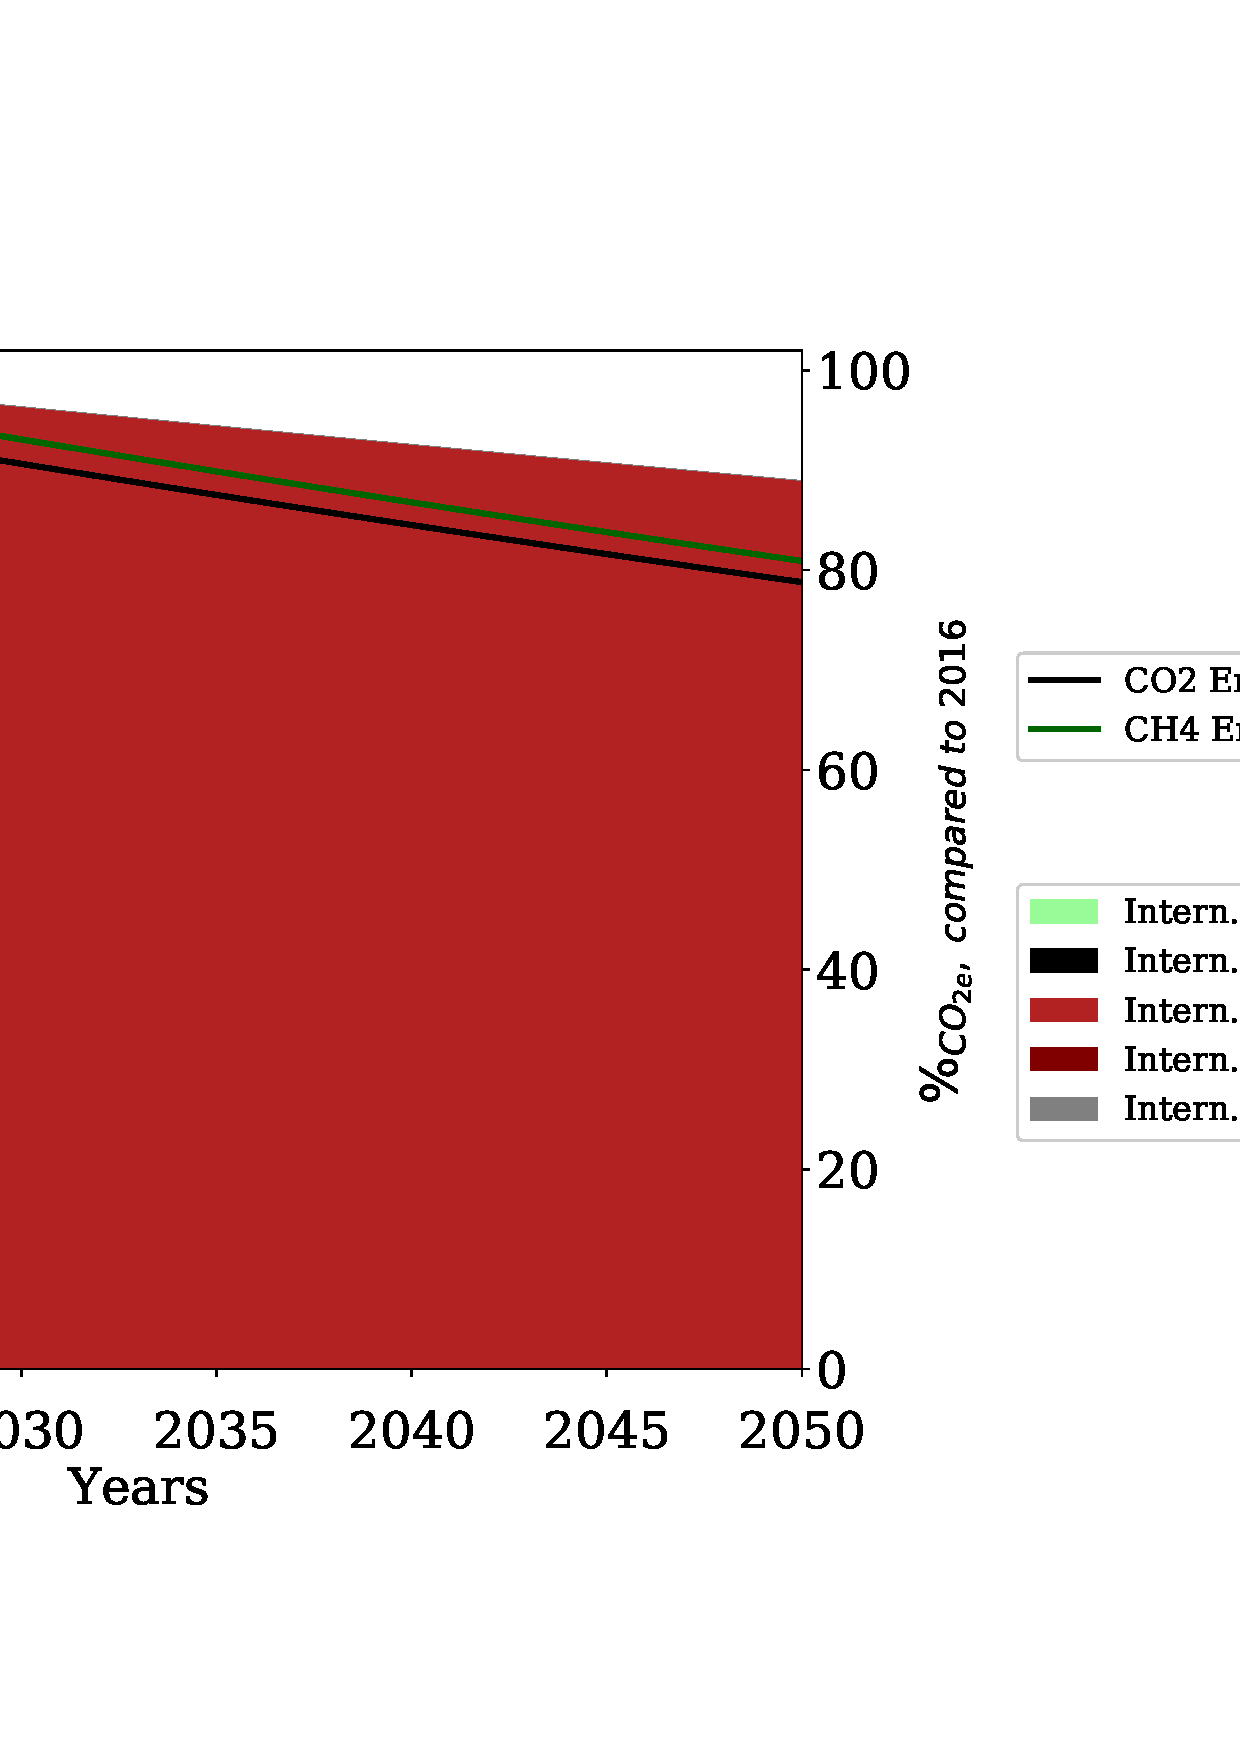
\includegraphics[width=\textwidth]{figures/BAU_fuels_emissions.pdf}
    \caption{Fuel consumption (y-axis left) and cumulative emissions (y-axis right) in the Business-as-usual scenario without carbon budget}
    \label{fig:BAU}
    % TODO: Figure einfügen und am besten auf einer zweiten y-Achse die kumulativen Emissionen reinbringen. Die fuels vll. einfach in % angeben, falls das mit den 16PJ nicht mehr herauszubekommen ist.
\end{figure}

\begin{figure}
    \centering
    \includegraphics[width=\textwidth]{figures/IMO_fuels_emissions.pdf}
    \caption{Fuel consumption (y-axis left) and cumulative emissions (y-axis right) in the IMO scenario, applying the climate emission target of the International Maritime Organsiation for 2050}
    \label{fig:IMO}
    % TODO: Figure einfügen und am besten auf einer zweiten y-Achse die kumulativen Emissionen reinbringen. Die fuels vll. einfach in % angeben, falls das mit den 16PJ nicht mehr herauszubekommen ist.
\end{figure}

\begin{figure}
    \centering
    \includegraphics[width=\textwidth]{figures/RS_fuels_emissions.pdf}
    \caption{Fuel consumption (y-axis left) and cumulative emissions (y-axis right) in the Reference scenario with a limited carbon budget}
    \label{fig:REF}
    % TODO: Figure einfügen und am besten auf einer zweiten y-Achse die kumulativen Emissionen reinbringen. Die fuels vll. einfach in % angeben, falls das mit den 16PJ nicht mehr herauszubekommen ist.
\end{figure}

% REF compared to REF methane leakage?
The comparison between the REF scenario with a methane leakage phase out scenario (see \autoref{fig:RS_MP} illustrates the impact, methane emissions have on the possible application of LNG and LBG in a climate emission reduction regime.

\begin{figure}
    \centering
    \includegraphics[width=\textwidth]{figures/RS_MP_fuels_emissions.pdf}
    \caption{Fuel consumption (y-axis left) and cumulative emissions (y-axis right) assuming methane leakage phase-out}
    \label{fig:RS_MP}
    % TODO: Figure einfügen und am besten auf einer zweiten y-Achse die kumulativen Emissionen reinbringen. Die fuels vll. einfach in % angeben, falls das mit den 16PJ nicht mehr herauszubekommen ist.
\end{figure}

% Demand variation - Cheapest?, Cost reduction bigger than transport reduction
% aus Tills Arbeit: Since transport demand declines over time, less investments are needed so that the system costs fall by 25 % to 15 billion EUR2016. These overall cost reductions are much greater than the entire transport demand reduction of 17 %. The faster the demand curves in Fig. 8.12 fall before it reaches the year of major investments into new fuel technologies, the greater this cost benefit would be.


% Cost variation: Methanol and Ammonia are close
Due to the high level of uncertainty of cost development of infrastructure, fuel and propulsion technology of different marine fuel options, a wide range of cost variations is applied to test for its effect on fuel composition. The results are summarised in \autoref{fig:costVariation}. Depending on the cost rate change of a specific fuel technology (x-axis), while keeping all other parameters constant, its share in the total fuel consumption from 2016-2050 (y-axis) changes significantly. The black dashed line at a cost rate change of zero represents the reference scenario. Already at a 10\% cost change rate (including fuel, technology and infrastructure costs), methanol and ammonia respectively gain relevance, reaching a dominant role at a 20\% cost change rate. Thus if the costs of either methanol or ammonia drop by 20\%, these would take over the role of hydrogen as the main renewable fuel of the future.

% LNG is no option, LBG just if methane leakage phase out
For LBG, the development of the methane leakage problem is of outstanding importance. Under the assumption that methane leakage can be coped with until 2050 (dashed line), LBG is close to hydrogen, methanol and ammonia as choice to be the dominate fuel in 2050. Contrary to that, LNG would not only require a methane leakage phase out, but also a very favourable cost development to play a major role.

% BATW has to be decreased significantly, but the conditions applied were rather unfavorable for BATW.
Sailing cargo ships, driven by a combination of wind and electricity from batteries seem to only be cost efficient in case of very strong drops in costs. However, the influence factors have more dimensions than just the pure battery and ship costs. In this model, it is assumed that one third of the propulsion is done by electricity. For long distance cargo, that mainly has to use the engine for manoeuvring into and out of the harbour, the wind share and potentially additional solar input can be significantly increased and thus the required battery and electricity costs reduced.

\begin{figure}[t]
    \centering
    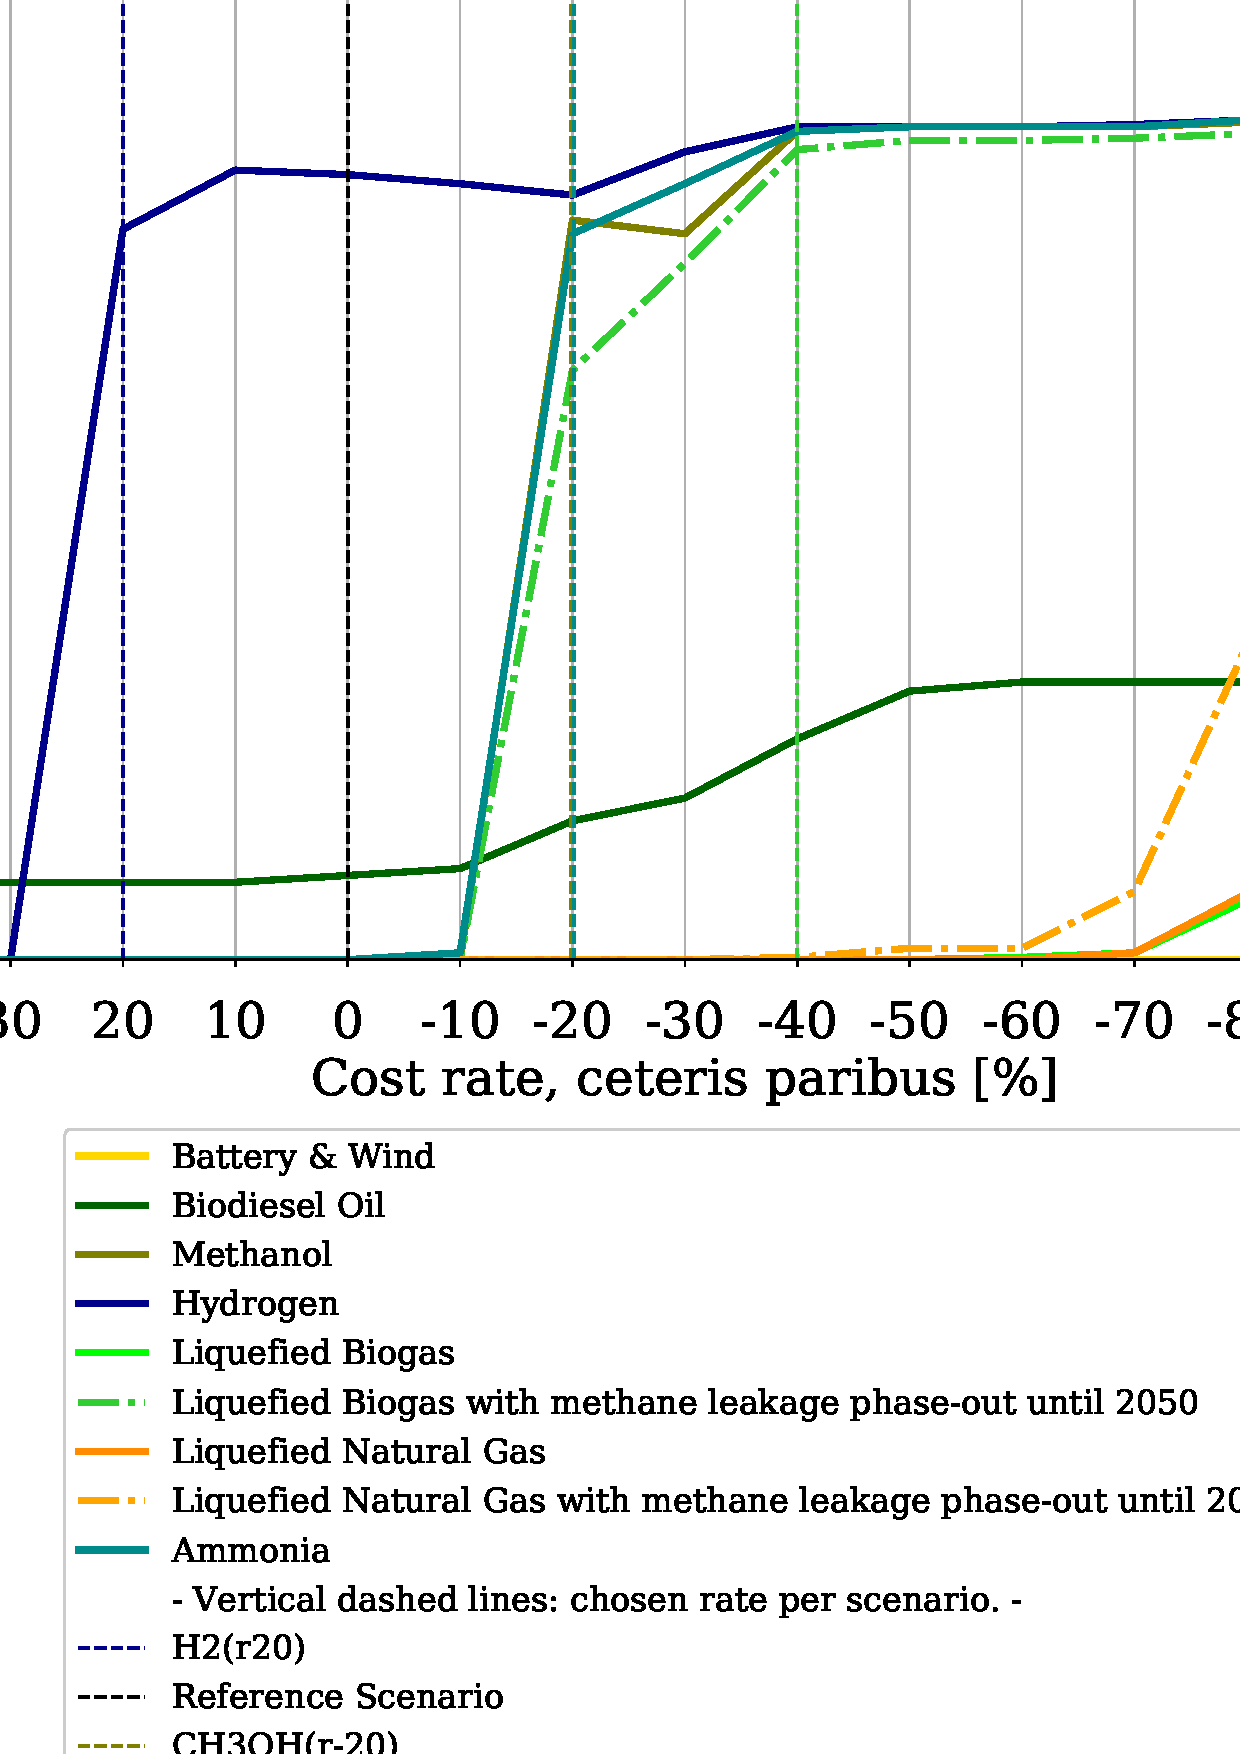
\includegraphics[width=.75\textwidth]{figures/costVariation.pdf}
    \caption{Total fuel shares from 2016-2050 (y-axis) in relation to different cost range changes (x-axis) compared to the reference case}
    \label{fig:costVariation}
    % TODO: Figure einfügen mit ausfuehrlicheren Fuel Namen
\end{figure}

% Compare all scenarios: Fuel composition total and 2050
For comparison, the total fuel use of all scenarios for 2016-2050 is displayed in \autoref{fig:AllFuelTotal} and the fuel composition in the target year 2050 in \autoref{fig:AllFuel2050}. A general efficiency increase can be seen for all carbon budget scenarios. Due to higher operational tank-to-propeller efficiency and thus a higher Tkm/GJfuel - rate, less fuel is applied in the carbon budget scenarios. Except the transport demand scenario all supply the same transport demand.

\noindent
\begin{minipage}[t]{0.49\textwidth}
    \centering
    \captionsetup{justification=centering}
    \captionof{figure}{Total fuel use from 2016-2050}
    \includegraphics[width=.95\textwidth]{figures/AllFuelTotal.pdf}
    \label{fig:AllFuelTotal}
\end{minipage}
\begin{minipage}[t]{0.49\textwidth}
    \centering
    \captionsetup{justification=centering}
    \captionof{figure}{Fuel composition in 2050}
    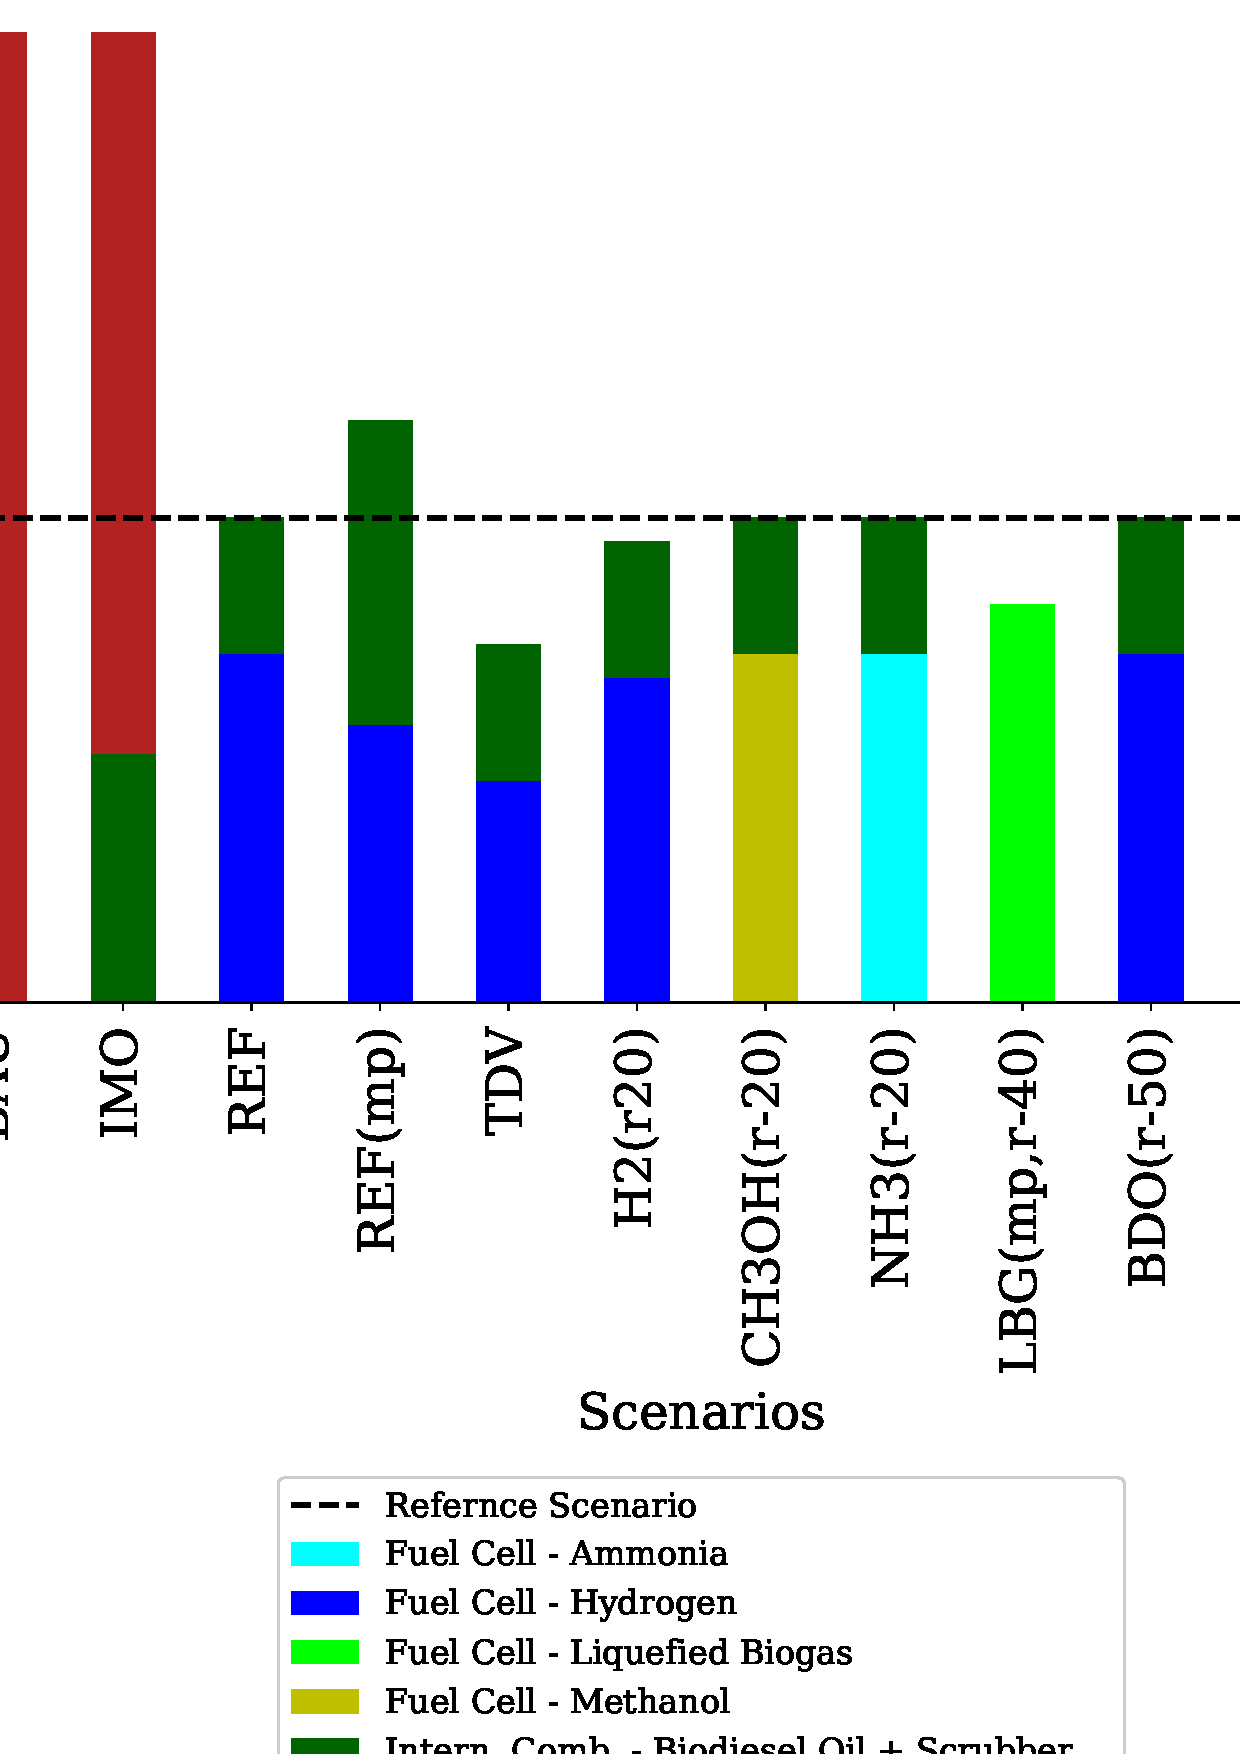
\includegraphics[width=.95\textwidth]{figures/AllFuel2050.pdf}
    \label{fig:AllFuel2050}
\end{minipage}\\[0.75cm]

% \begin{figure}[htb]
%     \centering
%     \includegraphics[width=.75\textwidth]{figures/AllFuelTotal.pdf}
%     \caption{Total fuel use from 2016-2050 for all scenarios}
%     \label{fig:AllFuelTotal}
%     % TODO: Figure einfügen mit ausfuehrlicheren Fuel Namen
% \end{figure}

% \begin{figure}[htb]
%     \centering
%     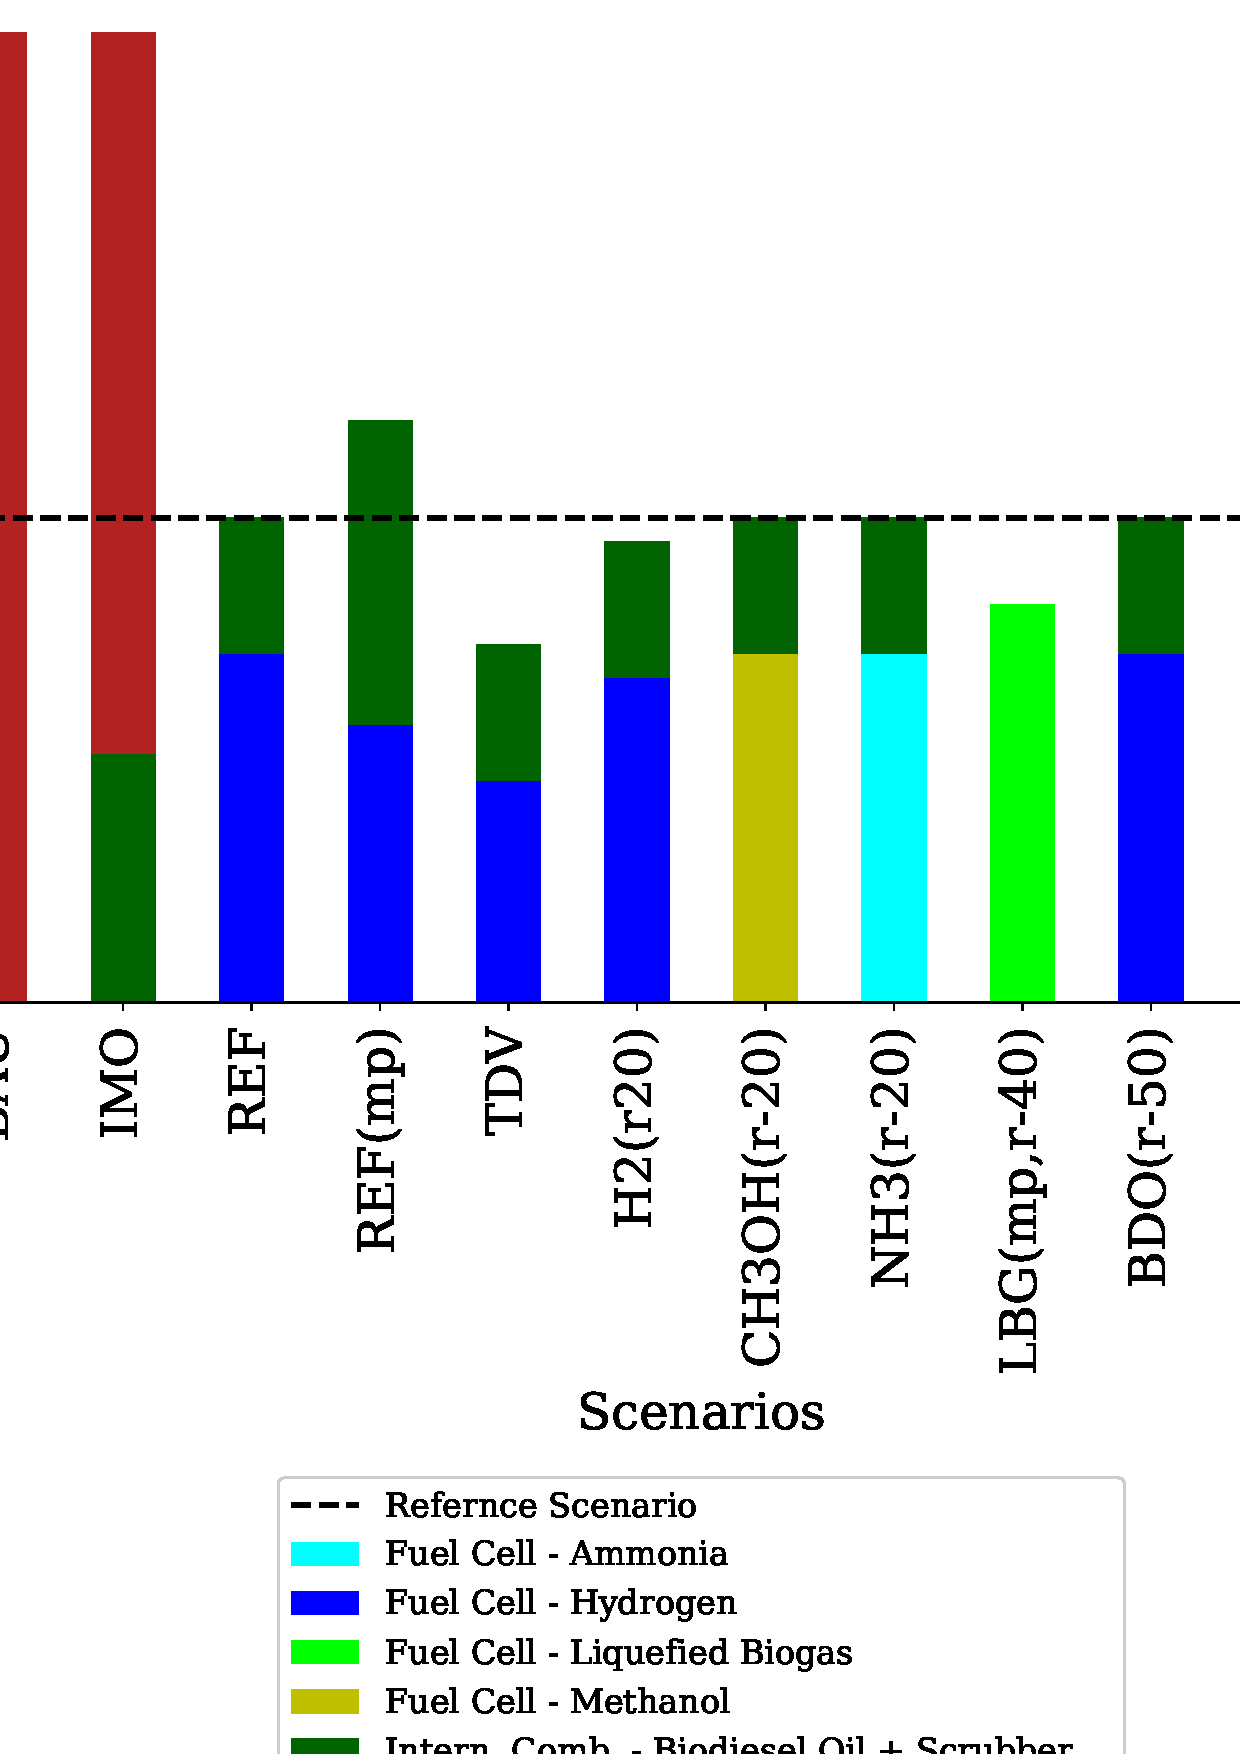
\includegraphics[width=.75\textwidth]{figures/AllFuel2050.pdf}
%     \caption{Fuel composition in 2050 for all scenarios}
%     \label{fig:AllFuel2050}
%     % TODO: Figure einfügen (die hab ich bisher noch nicht gesehen, hoffe die ist nicht kompliziert zu machen?) EVENTUELL BEIDE GRAFIKEN NEBENEINANDER UND DAMIT IN EINE PACKEN
% \end{figure}

% Compare all scenarios: Costs - not sure if there should be a figure - maybe rather include the full table of results

% Costs - resulting EURO/CO$_2$e
Derived from the cost differences for fuel, ship and infrastructure, a carbon price in the range of 350--450 \euro(2016)/ton CO$_2$e would be required for a renewable transition of the Danish shipping sector. \citep[p.197]{Raucci2017} reports similar prices of around 430 \$(2013)/ton CO$_2$ for a global transition.

% applicability of the model on other countries
% applicability of the findings for the world shipping
The model code and most of the data references and pre-processing can also be applied for other countries, especially Europe. However, since shipping has a global perspective, the case study for Denmark already gives a good indication of the fuel shares chosen for a cost-optimal path to carbon neutrality in 2050 for the worldwide shipping. Conditions for shipping are similar, the basic parameters, technology, fuel and infrastructure costs are considered as world prices rather than reflecting local particularities. This is also reflected and validated by the similar CO$_2$e-cost range compared to other, worldwide studies. 

% Why the mentioned costs are rather the upper end
Compared to other sectors like electricity and heat, these mitigation costs per /ton CO$_2$e seem high, one has to consider several points. First, this is the upper bound of cost: Technologies considered are all applicable today, developments in other sectors applying similar fuel switch options could further increase costs, additional alternatives could evolve. Second, as shown in the demand reduction scenarios, any decrease in transport demand would save costs even beyond the proportional saving. This is due to not only fuel savings (proportional) but, also due avoided investments in new ships (disproportionate). And third, refits and hybrid solutions have not been considered to a great extent in the model functionality and could further decrease costs and ease the shift to different fuels.

% Costs - what does that mean for the cargo cost

% Co-benefits.
Thus, costs could get lower for the transition, but the question is also whether to talk about mitigation costs. Co-benefits like reduced air pollution have not been quantified on a monetary basis in the model and were this not part of the optimisation. However, these could have essential health benefits, maybe even reaching mitigation gains instead of mitigation costs.

% Regulation / Recommendations
The necessary transition will not happen under current market conditions. Regulation is required urgently to bring shipping on the pathway to carbon neutrality in 2050, in line with the Paris Agreement. A carbon budget for shipping worldwide, broken down to countries is a viable option to consider. Additionally research money for alternative fuels and technologies, as well as solving crucial questions on security, infrastructure and methane leakage issues are important contributions to implement the transition to climate neutral shipping in 2050. 

% might be missing: strengths ad weaknesses of te model.
% Could also be added in the discussion: Important to model this in connection to the whole energy system, has effects!!

\section{Conclusion}
\label{sec:Conclusion}
% 250 words
% only draft until now!
The achievement of CO$_2$-neutrality in the shipping sector is of great importance for reaching the targets of the Paris Agreement. Although this goal is underrepresented in the current discussion, this study shows, that it is possible for the Danish part of international shipping to become CO$_2$-neutral until 2050 with existing technologies. Regarding fuels, hydrogen, methanol and ammonia are from a socio-economic cost perspective the most compatible. Due to high uncertainties regarding future cost developments and safety requirements (esp. ammonia), there is no clear winner. Regarding technologies, fuel cells are chosen for these fuel options, the decisive parameter being the higher fuel efficiency. Although LNG is the fuel option most prominently discussed as an alternative today, it would only have a short window of opportunity, mainly because of leakage problems of methane causing high greenhouse gas emissions as well as high fuel and technology costs. If this gaseous fuel is based on renewable sources, the so-called LBG can only play a role if methane leakage can be drastically reduced until 2050. The option of cargo-ships driven by a mixture of wind and electricity stored in batteries could not adequately be represented in the model setting. The evaluation of their role would need a further refinement of the calculations.
%Although additional conditions for the future application of fuel for shipping like safety issues or infrastructure decisions are not reflected in the model, ...
The presented modelling approach indicates that either strong regulative carbon budgets or a carbon price of 350--450 \euro/t~CO$_2$e would be required to induce the necessary changes for a carbon neutral Danish shipping in 2050. This would double today's average cargo transport costs. However, due to the low share of transport cost on the value of transported goods, the average transported good would only increase by 6\% on average. This can be considered as the upper limit, since new fuel possibilities not reflected in this study might evolve.

\section*{References}

\bibliography{mybibfile}

\end{document}